%\chapter{Длинное название главы, в которой мы смотрим на примеры того, как будут верстаться изображения и списки} \label{chapt2}


\chapter{Определение позы камеры}

В данной главе я предлагаю метод определения позы камеры, основанный на анализе размеров изображений объектов интереса в наблюдаемой сцене. Предложенный метод имеет два ключевых отличия от предыдущих:
\begin{enumerate}
\item учитывает ложные обнаружения объектов интереса в сцене и неточности локализации присутствующих объектов;
\item предсказывает положение камеры даже при значительных углах её наклона.
\end{enumerate}

Позой камеры называется положение и направление съемки камеры относительно сцены. Таким образом, для определения позы камеры необходимо выбрать систему координат, связанную со сценой, называемую в дальнейшем мировой.

С камерой также связанна система координат. Для обозначения её базисных векторов в данной работе я использую $x_c$, $y_c$ и $z_c$. Начало координат камеры находится в её оптическом центре, $x_c$ совпадает с направлением вправо на изображении, а $y_c$ "--- с направлением вниз. Направление $z_c$ называется направлением камеры. Её положением является положение её оптического центра. Таким образом, поза камеры задает преобразование мировой системы координат в систему координат камеры.

Для дальнейшего описания предложенного метода следующем разделе я представляю модель наблюдаемых данных.

\section{Математическая модель наблюдаемых данных}  \label{chap-cam_pose::sec-model}

В данной работе я предлагаю модель наблюдаемых данных состоящих из плоской статичной сцены и людей, находящихся в ней. Такая аппроксимация подходит для описания большинства сценариев видеонаблюдения. Ниже я предлагаю описание трёх её составляющих моделей: сцены, камеры и человека.

\subsection{Модель сцены}

Под сценой в данной работе я подразумеваю неподвижные объекты, изображения которых получает камера. Таким образом сцена может состоять из дорог, зданий, деревьев, скамеек и др. Поскольку предлагаемый метод не использует семантическую информацию об объектах сцены, то в данной работе я рассматриваю простейшую модель сцены, состоящей из единственной горизонтальной плоскости "--- плоскости земли.

Для задания позы камеры необходимо выбрать мировую систему координат, связанную со сценой. Я использую $x_w$, $y_w$ и $z_w$ для обозначения её базисных векторов. Мировая система координат выбрана таким образом, что плоскость земли совпадает с плоскостью $z=0$, а вектор $z_w$ совпадает с направлением вверх в сцене. В качестве начала мировой системы координат я выбрал проекцию положения камеры на плоскость земли.

В данной работе я предполагаю, что скалярное произведение $y_c$ и $z_w$ отрицательно, т.е.~изображение не перевернуто, а вектор $x_w$ коллинеарен проекции вектора $z_c$ на плоскость земли. Описанные ограничения однозначно определяют мировую систему координат в наблюдаемой сцене.

\subsection{Модель камеры}

Я использую модель перспективной проекции, которая описывается фокусным расстоянием камеры $f_c$. Физические характеристики используемой камеры также описываются несколькими параметрами: размером матрицы камеры $w_c, h_c$, положением принципиальной точки $(x_c, y_c)$, размерами пикселя $(w_p, h_p)$ и углом его скоса $\alpha_c$. Я использую предположение камеры с квадратными пикселями ($w_p = y_p$, $\alpha_c$), принципиальная точка которой располагается в центре изображения ($x_c = \frac{w_c}{2}$, $y_c = \frac{h_c}{2}$).

При заданных ограничениях модель перспективная проекция полностью определяется матрицей внутренней калибровки камеры, которая имеет следующий вид:
\begin{equation}
	K = \left[
	\begin{matrix}
		f & 0 & w_I \\
		0 & f & h_I \\
		0 & 0 & 1
	\end{matrix} \right]
\end{equation},
где через $f = \frac{f_c}{w_p}$ "--- фокусное расстояние, вычисленное в размерах пикселя, а $(w_I, h_I)$ "--- размер изображения.

\subsection{Модель человека}

Единственными движущимися объектами в сцене являются люди. Я использовал модель человека, предложенную в статье \cite{pishchulin15arxiv}. Она является отображением параметров позы и комплекции в положение вершин трехмерной модели человека.

\section{Поза камеры}

Выбранная модель сцены однозначно определяет взаимное положение мировой системы координат и системы координат камеры. При заданных ограничениях поза камеры $l_{c}$ однозначно определяется тремя параметрами:
\begin{itemize}
	\item высотой $h$ камеры над плоскостью земли;
	\item углом $t$ наклона камеры;
	\item углом $r$ поворота камеры.
\end{itemize}

Высота $h$ камеры над плоскостью земли определяет положение оптического цента камеры на оси $z$. Углы наклона $t$ и поворота $r$ камеры являются углами нутации и собственного вращения при преобразовании мировой системы координат в систему координат камеры.

Формально задача определения позы камеры по изображению имеет следующий вид:
\begin{itemize}
\item[\textbf{Вход:}]
\begin{itemize}
\item Последовательность $\left\{I_t\right\}_t^T$ изображений, полученная статичной камерой;
\item Фокусное расстояние $f$ камеры;
\end{itemize}
\item[\textbf{Выход:}] Параметры позы камеры в сцене: $l_{c} = \left( h, t, r \right)$.
\end{itemize}

Алгоритм может быть использован для последовательностей, содержащих  как цветные, так и монохромные изображения произвольного размера. На наблюдаемые данные накладываются следующие ограничения:
\begin{itemize}
	\item в данный представлено не менее трех изображений людей, не расположенных на одной прямой;
	\item изображения голов людей имеют размер не менее $16\times16$ пикселей;
	\item высота $h$ камеры не превосходит 20 метров;
	\item угол поворота $r$ камеры находится в пределах $\left(-\frac{\pi}{12}, \frac{\pi}{12}\right)$;
	\item фокусное расстояние $f$ камеры ограничено $5000$ размерами пикселя.
\end{itemize}

Входная последовательность изображений может иметь произвольный размер, в частности содержать единственное изображение.

\section{Предложенный метод}

Я разработал метод определения позы камеры, основанный на анализе размеров изображений объектов интереса в наблюдаемой сцене. В качества объектов были выбраны головы людей, поскольку в отличие от фигур всего человека они меньше подвержены перекрытиям в сценарии видеонаблюдения.

Для построения отображения входного изображения в параметры камеры я использовал методы машинного обучения с учителем. В связи с отсутствием больших размеченных коллекций с известными положениями объектов и камеры в сцене обучение происходило на синтетической выборке.

\subsection{Построение обучающей выборки}

Обучающая выборка состоит из синтетических последовательностей изображений. Для её построения я использовал модель наблюдаемых данных, описанную в разделе \ref{chap-cam_pose::sec-model}.

Алгоритм оценки позы камеры использует только положение и размер головы человека на изображение. Поэтому в синтетической выборке не моделируется разнообразие поз людей реального мира, и все люди находятся в стандартной позе. В качестве роста людей в сцене я выбрал 1.75 метра "--- средний рост взрослых европейцев.

При построении выборки изображения не удовлетворяющие ограничениям модели наблюдаемых данных отбраковывались. Построенная синтетическая выборка состоит из 100373 последовательностей, содержащих по 300 изображений в среднем. Каждое изображение содержит оного человека расположенного в произвольном месте изображения. Таким образом удается добиться того, что каждый человек хорошо виден на изображении.

\subsection{Выбор признакового описания}

Синтетические последовательности изображений визуально отличаются от реальных данных. Поэтому для обучения алгоритма регрессии позы необходимо выбрать признаковое описание инвариантное к используемой выборке.

В качестве описания я использую результаты обнаружения голов людей на изображении. Таким образом, каждый человек на изображении описывается тройкой чисел $\left(x_h, y_h, s_h\right)$, соответствующей положению центра его головы и её линейным размерам. Конечно, модель человека \cite{pishchulin2015building} позволяет определить реальное положение головы человека на синтетическом изображении. Однако, мы не можем применить тот же метод оценки положения головы человека к изображения реальных данных. Поэтому при использовании разных способов оценки положения головы человека на реальных и синтетических данных может возникнуть проблема оценки построенного алгоритма определения позы камеры. Поэтому я использовал метод локализации объектов на изображении даже к синтетическим данным. Такой подход позволил мне учесть небольшие ошибки в локализации и определении размеров алгоритмом локализации головы человека. Также этот подход позволяет использовать для определения позы камеры любые объекты, для которых доступна модель и алгоритм локализации на изображении.

Для локализации голов людей на изображении был выбран алгоритм \cite{prisacariu_reid_tr2310_09} и использована его оптимизированная версия \footnote{https://bitbucket.org/13e\_sha/fasterhog}. Использование данного алгоритма обусловлено высокой скоростью его работы. Этот фактор оказался очень важным для построения большой коллекции изображений синтетической выборки. Также данный алгоритм не чувствителен к наличию текстуры на изображении человека.

Для построения прецедента для обучения алгоритма регрессии позы камеры я использовал информацию о 64 людях в сцене. 

\subsection{Регрессия позы камеры}

Я использовал сверточную нейронную сеть для оценки позы камеры.

Важно отметить, что точность предсказания должна зависеть от позы камеры. При увеличении высоты камеры над плоскостью земли, точность её предсказания может уменьшаться. Таким образом, разные последовательности выборки могут иметь различную сложность при обучении.

Я учел это предположение в функции ошибки построенной нейронной сети. При решении задачи регрессии обычно используют Евклидову функцию потерь. К сожалению, она одинаково ``штрафует'' отклонение от правильного ответа для всех прецедентов. Для решения этой проблемы в качестве функции потерь я использовал взвешенную сумму квадратичных отклонений, где значение параметра и вес его вклада предсказывается нейронной сетью.

Формально, построенный алгоритм использует предположение нормального распределения позы камеры $l=\left( h, t, r \right)$ при условии наблюдаемых признаков сцены $x$ и  предсказывает математическое ожидание $\tilde{l_c}$ и дисперсию $\Sigma_c$ этого распределения: 
\begin{equation}
p(l_{c}|x, \Theta) = N(l_c|\tilde{l_c}(x, \Theta), \Sigma_c(x, \Theta))
\end{equation}

Матрица ковариации $\Sigma_c$ должна быть положительно определенной. Я учел это ограничение в функции потерь, добавив предположение о независимости параметров позы камеры. Также нейронная сеть предсказывает логарифм элементов матрицы ковариации:
\begin{equation}
	\Sigma_c(x, \Theta) = diag\left(e^{s(x, \Theta)}\right) + \epsilon I,
\end{equation}
где $s(x, \Theta) = \left( s_h(x, \Theta), s_t(x, \Theta), s_r(x, \Theta) \right)$ "--- вектор параметров матрицы ковариации. Параметр регуляризации $\epsilon$ был выбран равным $10^{-6}$.

Параметр $\lambda_c = \left|\Sigma_c^{-1}\right|$ можно интерпретировать как уверенность алгоритма в предсказании. Важно отметить, что в предложенном методе этот параметр зависит от наблюдаемых данных $x$.

В качестве функция потерь был выбран отрицательный логарифм правдоподобия наблюдаемых данных:
\begin{equation}
L(\left\{l_c\right\}_i | \left\{ \tilde{l_c^i} \right\}_i, \left\{s^i\right\}) = -\sum_i\log N(l_{c}^i|\tilde{l_c^i}, diag\left(e^{s^i}\right) + \epsilon I)
\label{eq:norm}
\end{equation}

\begin{figure*}[!t]
	\centering
	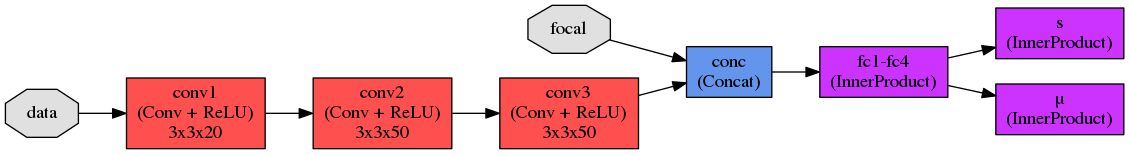
\includegraphics[width=\textwidth]{camera_pose/1}
	\caption{Схема использованной нейронной сети для предсказания параметров позы камеры.}
	\label{fig:net}
\end{figure*}

Производные используемой функции потерь могут быть вычислены аналитически:
\begin{align}
	\frac{\partial L}{\partial \tilde{\l_c^j}} &= 
	\frac{\tilde{\l_c^j} - l_c^j}{e^{s^j} + \epsilon}
	\label{eq:der_mu} \\
	\frac{\partial L}{\partial s^j} &= 
	\frac{1}{2}\frac{e^{s^j}}{e^{s^j} + \epsilon}
	\left(1 - \frac{(\tilde{l_c^j} - l_c^j) ^ 2}{e^{s^j} + \epsilon}\right)  \label{eq:der_sigma}
\end{align}

Выражения \eqref{eq:norm}, \eqref{eq:der_mu} и \eqref{eq:der_sigma} допускают эффективную реализацию используемой функции потерь на современных графических ускорителях.

Я использовал сверточную нейронную сеть прямого распространения. Входом нейронной сети является тензор размера $3\times8\times8$, описывающие положение и размер каждой из 64 обнаруженных голов. Чтобы алгоритму не потребовалось адаптироваться ко всевозможным перестановкам объектов прецедента, они были отсортированы по возрастанию размера.

Построенная нейронная сеть состоит из 3 сверточных слоёв, после которых используется нелинейная функция ReLu. Размер каждой сверки равер $3\times3$. Такой подход позволяет сверточным слоям 1) использовать информацию об удаленных объектах, размер которых существенно отличается и 2) адаптироваться к шуму в данных за счет использования объектов, чьи размеры отличаются слабо.

После применения сверточных слоёв полученный результат объединяется с фокусным расстоянием $f$ камеры и подается на вход полносвязным слоям. Описанная выше функция потерь позволяет обучать нейронную сеть предсказывать положение камеры и уверенность предсказания.

\subsection{Объединение результатов прецедентов}

Построенная нейронная сеть предсказывает позу камеры, используя положения не более 64 людей в сцене. Во реальных сценариях видеонаблюдения количество людей в сцене может существенно превышать это значение. Поэтому необходимо предложить метод объединения результатов на разных наборах данных.

Для решения этой проблемы можно объединить результаты работы алгоритма на $K$ разных подмножествах обнаружений людей с помощью наивного Байессовского метода:
\begin{align}
	\overline{l_c} &= \overline{\Sigma_c} \left( \sum_k^K{\Sigma_{c,k}^{-1} \tilde{l}_{c,k} } \right) \\
	\overline{\Sigma_c} &= \left( \sum_k^K \Sigma_{c,k}^{-1} \right) ^ {-1},
\end{align}
где $\overline{l_c}$ "--- предсказанная поза камеры.

Важно отметить, что данных подход может быть применен только при отсутствии зависимости между предсказанными позами камеры на разных подмножествах данных. Чтобы этого добиться, можно использовать непересекающиеся подмножества обнаружений объектов на разреженном подмножестве кадров.

To make the final solution we choose a distribution with the smallest differential entropy. For Gaussian distributions it also has the smallest determinant of the predicted covariance matrix $\Sigma$. The mean value of the chosen distribution is the predicted location of the camera. We show the chosen distribution in the second row of рисунка~\ref{fig:bestClear}. Рисунок~\ref{fig:TownCentre_calibration} presents synthesized people on the real image from the video sequence. We see that the presented and synthesized people have similar sizes. Thus the proposed model predicts plausible camera location. In further experiments we use the predicted camera height as the groundtruth.

\begin{figure*}[!t]
	\centering
	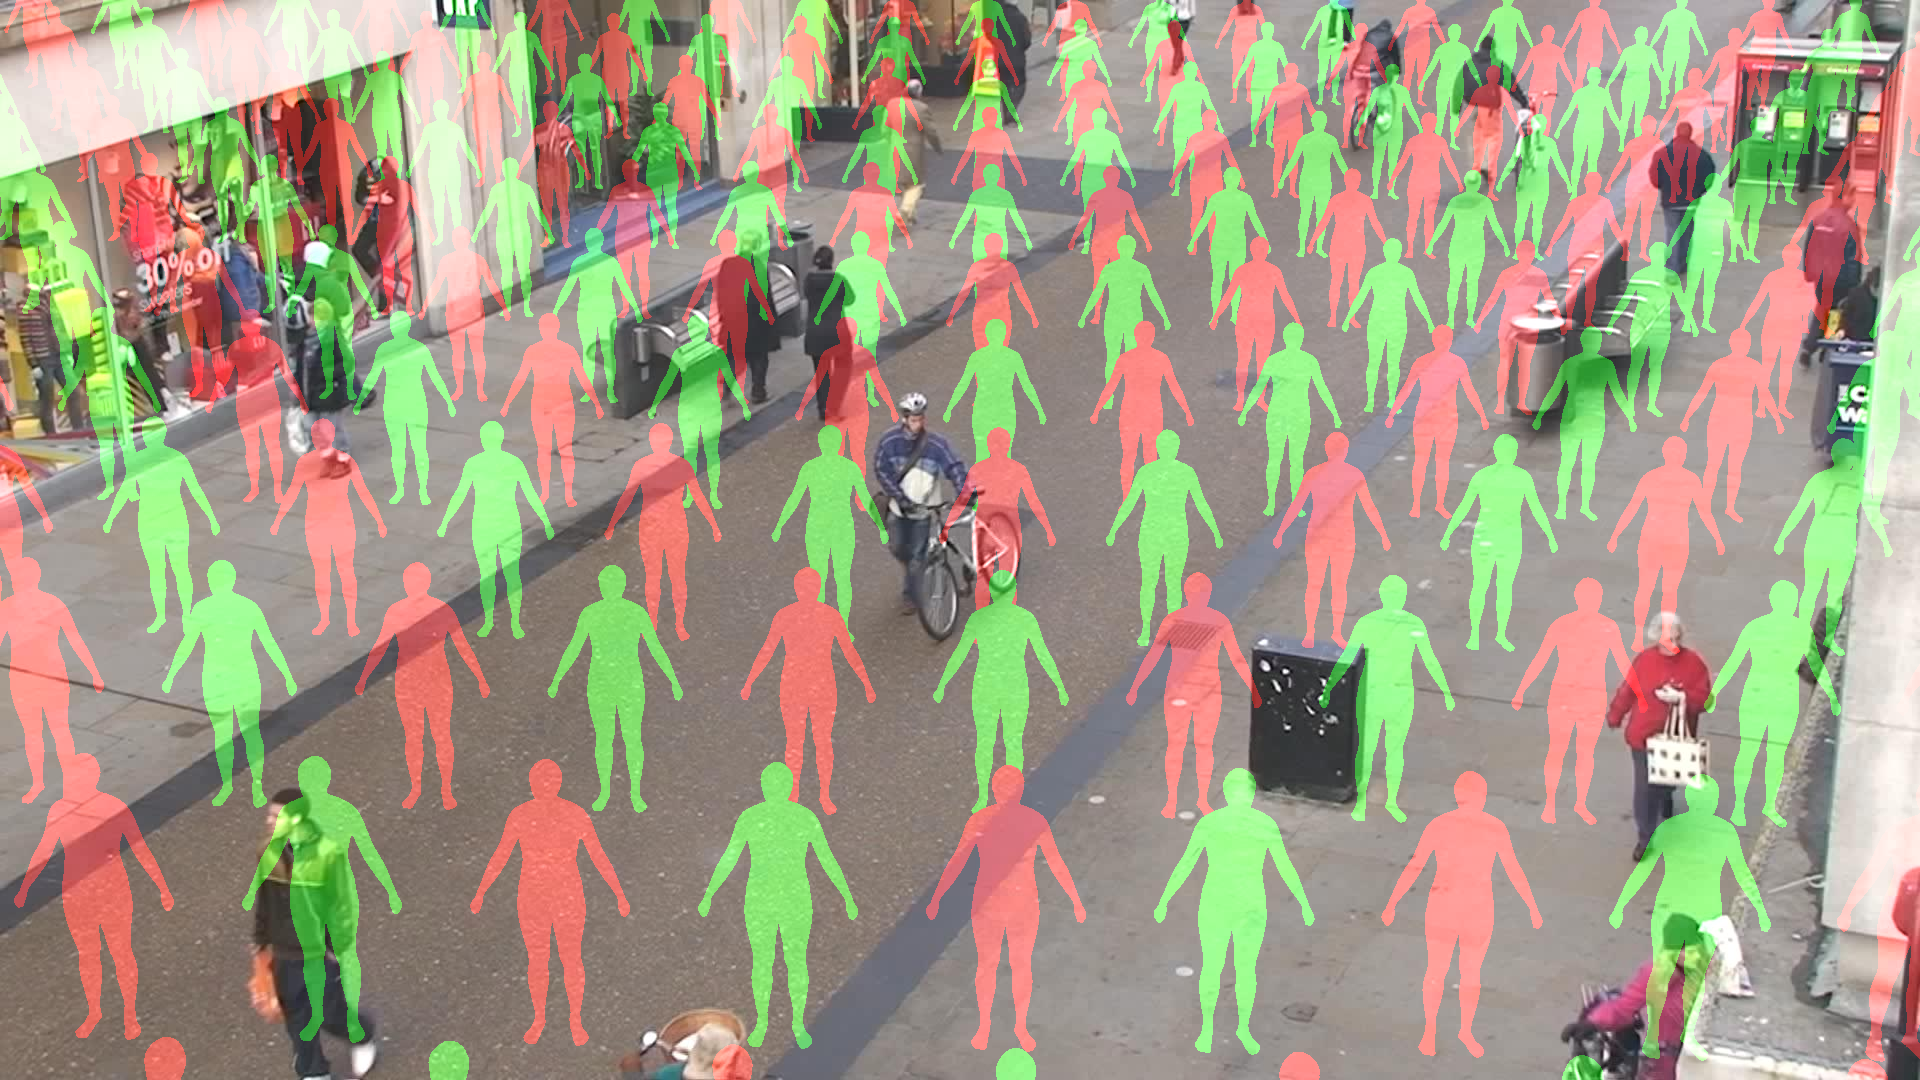
\includegraphics[height=72mm]{camera_pose/TownCentre_1}
	\caption{Визуализация синтезированных людей на предсказанной плоскости земли.}
	\label{fig:TownCentre_calibration}
\end{figure*}

In the next experiment we use all head detections on the TownCentre dataset. We repeat the proposed calibration technique used for clear detections. Note, that in average a number of false positives in the constructed samples are much higher than in train samples (52\% vs 10\%). The constructed results are shown in the third row of \ref{fig:bestClear}. It shows that the predicted camera location is close to its true value even when there are a huge number of false positive detections.

In addition we experiment with duplicate detections in a sample. We choose a single true positive head found by the detector and construct a sample that contains 64 copies of this head. Such an extreme case of duplication corresponds to a scene with a single person standing in the same place for a long time. Camera location cannot be predicted from this sample as is it specifies only distance to the single person in a scene. Рисунок~\ref{fig:bestClear} shows that the model predicts a very significant error for camera locations that can produce such a detection. Thus a determinant of the predicted covariance matrix is a good measure of the model confidence.

Our training data assumes that people can be found in each location of the input images. Thus, each training sample contains people uniformly distributed in the image plane. Hence, the long input video sequence is preferable as it gives better statistics of people sizes across image plane.

We evaluate the proposed method on four video sequences of the more challenging PETS 2006 dataset \cite{thirde2006overview}. It's important to notice, that the first and second video sequences of this dataset violate our assumption of a single ground plane. These video sequences contain people on several floors. Nevertheless, we apply the proposed method to all video sequences in the dataset and use all detector results as the features. Our evaluation (см. таблица~\ref{tab:PETS}) reveals that the proposed method correctly estimate camera location on the third and fourth sequence and cannot predict plausible camera pose on the first two sequences. However the predicted deviation is significantly larger for such failure cases, thus the model indicates low confidence in these predictions.

\section{Обучение и экспериментальная оценка}

В этом разделе я опишу используемый метод обучения параметров построенного алгоритма и результаты его тестирования на синтетических и реальных данных.

\subsection{Обучение}

Обучение нейронной сети проводилось на построенной синтетической выборке. Данная выборка содержит только верные обнаружения голов людей. Эксперименты показали, что обучение на таких ``чистых'' данных не позволяет алгоритму обобщаться на обнаружения, содержащие ошибки.

Для решения этой проблемы я промоделировал два типа шума в реальных данных: 1) ложные обнаружения голов в сцене; 2) дублирующиеся обнаружения в прецеденте. Второй тип шума может возникать, если человек неподвижен на нескольких кадрах. Для моделирования шума был применен следующий алгоритм:
\begin{enumerate}
	\item из множества обнаружений последовательности выбиралось подмножество из $n: 0 < n \le 64$ элементов;
	\item среди выбранных обнаружений $m: 0 < m < \frac{n}{10}$ произвольных заменялись на ложные срабатывания детектора со случайным положением и размером в сцене;
	\item из построенного множества производилась выборка 64 обнаружений с повторениями.
\end{enumerate}

Такой подход позволил промоделировать ложные срабатывания алгоритма локализации людей и дублирование обнаружений на разных кадрах. По каждой последовательности обучающей выборки было построено 3 прецедента.

Предложенная сверточная нейронная сеть имеет всего 67393 параметра и относительно небольшие размеры промежуточных слоёв. Это позволило сформировать батчи состоящие из 32768 прецедентов при обучении с помощью градиентного спуска. Скорость обучения понижалась по степенному закону с параметром $\gamma=0.95$ каждые 1500 итераций. Обучение заняло 200000 итераций. Я использовал 80\% последовательностей синтетической выборки для обучения и 20\% для валидации.

Важно отметить, что из-за использования алгоритма локализации объектов на изображении, обученные параметры нейронной сети чувствительны к смене алгоритма локализации объектов. Таким образом, при его замене необходимо повторное обучение.  С другой стороны, предложенный подход позволяет отказаться от моделирования неточностей в локализации объектов используемым алгоритмом. Более того, при его замене обученные параметры нейронной сети могут являться хорошим начальным приближением.

\subsection{Экспериментальная оценка на синтетической выборке}

Я провел несколько экспериментов для оценить качество построенного алгоритма. 

Первый эксперимент показывает влияние размера обучающей выборки и количества полносвязных слоёв на качество построенного регрессора (см.~таблицу \ref{part2::arch}). Поскольку 

 В первую очередь было проведено тестирование на синтетической валидационной выборке. Визуализация ошибки на тренировочной и валидационной выборке показало, что не происходит переобучение алгоритма к тренировочной выборке.

\begin{table} [htbp]
	\caption{Зависимость средней нормализованной ошибки на обучающей и валидационной выборках}\label{part2::arch}%
	\begin{tabulary}{\textwidth}{@{}>{\zz}L >{\zz}C >{\zz}C >{\zz}C}
		\hline
		Размер выборки (последовательностей) & Количество полносвязных слоёв & Средняя ошибка на обучении & Средняя ошибка на валидации\\
		\hline
		20448 & 3 & 0.1061 & 0.121 \\
		20448 & 4 & 0.0956 & 0.1167 \\
		20448 & 5 & 0.07 & 0.12 \\
		30179 & 4 & 0.09015 & 0.117 \\
		51366 & 4 & 0.09836 & 0.1064 \\
		80298 & 5 & 0.09764 & \textbf{0.1009} \\
		\hline
	\end{tabulary}
\end{table}


We perform several tests to evaluate quality of the constructed model. First of all we test our model on the synthetic validation set. Training process (рисунок~\ref{fig:training}) shows that error rate on training and validation sets are similar, i.e.\ the model does not overfits to training data.

\subsection{Экспериментальная оценка на реальных данных}

\section{Идея}


\section{\uppercase{Introduction}}
\label{sec:introduction}

\noindent Automatic extraction of useful information from a video is the key computer vision task. Location and attributes of presented objects as well as action they perform are the most interesting parts of such information.

If scene geometry and camera pose are known then these tasks become easier. Indeed, such information restricts available object locations. For example, cars usually can be found on the roads and their size on an image are restricted by the camera location and orientation, i.e.~ it's pose. On the other hand, modern object detection algorithms assume unknown scene geometry and camera pose. Therefore, they have to search objects of any size at all locations. It leads to false detections and high computation time. If only camera calibration is known we can reduce influence of these factors.

Unfortunately, in practice it is hard to estimate camera calibration parameters. The most robust methods require interaction with a calibration template. It makes calibration of hundreds of thousands of surveillance cameras intractable. In this paper we propose an algorithm that automatically solves this task for surveillance cameras with known focal length. Our algorithms don't require any special calibration templates and directly infer parameters from surveillance video. The constructed algorithm takes object detector results as the input.

We apply supervised machine learning to solve calibration task. Requirement of huge labeled dataset restricts implementation of machine learning techniques in practice. We show how to construct synthetic dataset to solve the calibration task. It allows estimation camera parameters even if there is no real labeled dataset at all.

We show that camera pose can be estimated from people observation in surveillance video. We construct a calibration algorithm that uses head detector results and known camera focal length as the input. As opposed to previous works in the area, we don't assume the "perfect" people detector and implicitly take into account its object localization error and false detections. Our algorithm makes the following assumptions about the observed scene:
\begin{enumerate}
	\item The camera is static, i.e.\ it does not change location, view direction and focal length;
	\item Camera observe "flat" scene, i.e.\ ground is a plane;
	\item All people stand on the ground plane;
	\item All people presented in the scene has the same height (1.75 meters).
\end{enumerate}
The assumption of a single flat ground plane is a standard for the works on surveillance calibration \cite{liu2011surveillance,chen2007accurate,dubska2014automatic,den2015automatic,micusik2010simultaneous}.

In real surveillance scenario camera produces continuous video stream and detector localizes thousands of objects per minute. In practice the set of detections contains false positives. Therefore, the calibration algorithm should a) work with input of various length and b) be robust to false positive. We show that the proposed calibration algorithm meets these requirements.

Our main contributions are:
\begin{enumerate}
	\item We propose a technique for construction a synthetic dataset for scene geometry understanding;
	\item We construct an algorithm for the camera pose estimation from people observation;
	\item The introduced algorithm is shown to be robust to noise in the input data and allows input of any length.
\end{enumerate}

\section{\uppercase{Related Work}}
\label{sec:related}

\noindent 

\section{\uppercase{Proposed Model}}
\label{sec:proposed}

\noindent We divide this section into several parts. In subsection \ref{sec:dataset} we propose a technique for synthetic dataset construction. Subsection \ref{sec:lognormloss} introduces our LogNormLoss layer for CNN that allows learning probabilistic prediction for regression tasks. In subsection \ref{sec:calibration} we propose an algorithm for camera calibration.

%------------------------------------------------------------------------- 
\subsection{Dataset}
\label{sec:dataset}

\noindent The proposed algorithm requires a labeled dataset for training. We found that it is hard to use real surveillance videos for this task. Most of such data does not contain calibration parameters and groundtruth people location. On the other hand, computer graphics allows construction synthetic dataset of an arbitrary size with specified parameters.

We construct synthetic dataset with 100373 scenes. Each scene is a ground plane with people standing on it and camera placed above. Scenes are differ in the intrinsic and extrinsic parameters of the camera and location of captured people. The proposed algorithm uses only head locations in form of bounding boxes and does not need original images. Thus our dataset contains 1) camera calibration parameters; 2) location of people on the ground plane and 3) head detector results. We describe used camera, human models and applied head detector below.

\subsubsection{Camera Model}

\noindent Camera calibration contains intrinsic and extrinsic parameters. World coordinate system specifies extrinsic parameters. Thus we choose an unified world coordinate system for all scenes. It specifies ground as a plane $z = 0$. We assume that a camera is placed on the Z axis. Therefore, the height $h$ is the only parameter of a camera location.

The view direction of the camera is specified by two angles: tilt $t$ and roll $r$ of the camera. These angles correspond to the second and third components of the Z-X-Z Euler angles. The first Euler angle is assumed to be zero as it specifies camera rotation around Z axis.

In the constructed synthetic dataset cameras record FullHD frames ($1920\times1080$). A principal point is assumed to be in the center of captured images and a camera has square pixels with aspect ratio equal to 1. In such assumptions the focal length $f$ (measured in pixels) is the only intrinsic parameter of the camera.

Each scene is parametrized by camera calibration parameters. We sample these parameters from uniform distributions with the boundaries specified in the таблице \ref{tab:params}.

\subsubsection{Human Model}

\noindent The only objects in our dataset are people and we apply human shape model~\cite{pishchulin2015building} to visualize them. Our dataset contains people in standard pose and constant shape. To make the dataset easier all people have the same height (1.75 meters). Thus only location on the ground plane specifies human shape.

We construct at least 200 people in different locations for each scene. We place each person in such a way that the applied detector could find him. In addition, we reject scenes where the detector cannot find people.

\begin{table} [htbp]
	\centering
	\captionsetup{width=15cm}
	\caption{Распределение параметров позы камеры в синтетической выборке.}\label{tab:params}%
	\begin{tabular}{|c|c|c|c|}
		\hline
		Parameter & Caption & Minimum value & Maximum value\\
		\hline
		\hline
		$h$ & height (m) & 0 & 20 \\
		$t$ & tilt (rad) & $\frac{\pi}{2}$ & $\frac{11\pi}{12}$ \\
		$r$ & roll (rad) & $-\frac{\pi}{12}$ & $\frac{\pi}{12}$ \\
		$f$ & focal length (pixels) & 0 & 5000 \\
		\hline
	\end{tabular}
\end{table}

\subsubsection{Detector}

\noindent We treat detector results as features extracted from a scene.
Modern person detectors are sensitive to camera angle and occlusions, therefore it cannot find people in some scenes. But heads are visible in most surveillance scenarios. Thus the proposed features consist of head bounding boxes.

Indeed, human model \cite{pishchulin2015building} provides the true head location in synthetic data. However, we apply the head detector even to synthetic images. It allows us to avoid modeling of the detector noise and bias in head localization. We assume that these factors are equal on real data and the proposed synthetic datasets. Thus the distributions of features extracted from the real and synthetic data becomes closer.

We use fast implementation \cite{prisacariu2009fasthog} of head detector. It has two significant advantages over the modern detectors: 1) low computation time of the detector allows construction the huge dataset in reasonable amount of time and 2) it finds heads even if we do not model texture of the person skin.

%------------------------------------------------------------------------- 
\subsection{LogNormLoss Layer}
\label{sec:lognormloss}

We use Convolutional Neural Network (CNN) to estimate the calibration parameters. The Euclidean loss is a traditional loss layer for such regression tasks. It assumes equal "penalty rules" for all predictions. In some cases it leads to inaccurate results. Imagine, the input data have outliers or huge noise level. A regression with the Euclidean loss tends to bias true predictions to compensate shift from groundtruth on such data. On the contrary, if the used model can indicate how "good" the input data are, it can overcome this drawback. The proposed LogNormLoss layer is a solution for this task. It estimates the predicted value and confidence of the prediction by minimizing negative logarithm of normal distribution density function.

Formally, LogNormLoss layer assumes that the true value $y$ is normally distributed with unknown mean $\mu$ and variance $\Sigma$:
\begin{equation}
p(y|x, \Theta) = N(y|\mu, \Sigma)
\end{equation}
It estimates the parameters $\mu$ and $\Sigma$ using maximization of the likelihood. If we assume that these parameters do not depend on the input data $x$, the layer describes all targets $y$ with a single Gaussian. On the other hand, CNN with LogNormLoss layer trains $\mu$ and $\Sigma$ as functions of the input data $x$ and model parameters $\Theta$.

The proposed loss layer has 3 inputs. The layer interprets first two inputs $\mu$ and $s$ as a mean and logarithm of a variance of normal distribution. Thus, the loss is a negative logarithm of a normal distribution density function:
\begin{equation}
L(y |\mu, s) = -\log N(y|\mu, e^{s} + \epsilon)
\end{equation}
We use $\epsilon = 1e-6$ to prevent overfitting to a single train sample.

If y is a vector we assume independence of the different components of the prediction:
\begin{equation}
L(y | \mu, s) = -\log N(y|\mu, diag\left(e^{s}\right) + \epsilon I)
\end{equation}

The $s$ parameter can be interpreted as a predicted error. The higher value it takes the fewer model confidence is. If the $s$ values are equal for all input data $x$, this loss equal to Euclidean loss. But if they depends on the observed data, CNN trains to estimate accuracy of the predicted mean value $\mu$ for the current input $x$.

Derivatives of the LogNormLoss layer has simple analytical form:
\begin{align}
	\frac{\partial L(y | \mu, s)}{\partial \mu_j} &= 
	\frac{\mu_j - y^j}{e^{s_j} + \epsilon} \\
	\frac{\partial L(y | \mu, s)}{\partial s_j} &= 
	\frac{1}{2}\frac{e^{s_j}}{e^{s_j} + \epsilon}
	\left(1 - \frac{(\mu_j - y^j) ^ 2}{e^{s_j} + \epsilon}\right) 
\end{align}

Equations \eqref{eq:norm}, \eqref{eq:der_mu} and \eqref{eq:der_sigma} allows efficient implementation of the layer for modern GPUs. We implement the LogNormLoss layer in the Caffe framework \cite{jia2014caffe}.

\subsection{Calibration Model}
\label{sec:calibration}

Our main goal is construction of calibration algorithm that predicts camera pose from people observations in the scene. It takes the bounding boxes of detected human heads and focal length (in pixels) as the input and predicts camera extrinsic parameters and confidence of the prediction.

We make several assumptions of the observed data. All people in the scene have the same height and stand on the ground plane. Thus all heads lie on a plane in a world coordinates. Therefore, if 3 found heads do not lie in a single line in the image, we can analytically estimate camera extrinsic parameters. Nevertheless, noise and quantization makes this solution inaccurate. Therefore, we construct each input sample from 64 head locations and solve the regression task using CNN.

The first problem we solve is how to present head detection to CNN. Initially the input head locations in a sample do not have any ordering. Hence, there are $64!$ permutations of the same head locations in a sample. If we use data without any ordering the constructed model should adapt to all of these permutations. To solve this problem we sort heads by size and arrange them in a grid. Consequently, the head locations forms a tensor of size $3\times8\times8$, where each head bounding box is presented by location of its top left corner and size.

The introduced structure of the sample allows us to use convolutional layers (см. рисунок~\ref{fig:net}). We apply 3 convolutional layers with ReLu non-linearity. Each convolution has size of $3\times3$. These layers allow 1) extract information from distant objects (correspond to convolution of columns) and 2) be robust to noise in data (convolution adjacent objects in a column).

After the third convolution and ReLu non-linearity we concatenate the constructed features with the camera focal length. The model applies five fully connected layers with non-linearity to this features. The model uses LogNormLoss layer to evaluate quality of the predicted camera location $\mu$ and its error $s$.

It is important to notice, as we use the detected bounding boxes, the proposed algorithm becomes sensitive to the applied detector, i.e.\ it fits to the detector. Thus, we should update synthetic dataset and repeat training of the CNN, if we want to use another detector. On the other hand, this solution allows us to skip modeling of the detector noise. Moreover, if results of another detector is similar to the ours, it is not necessary to train the model from scratch, the proposed CNN gives a good initialization.

%===========================================================
\section{\uppercase{Training and Evaluation}}
\label{sec:evaluation}

\begin{table*}[t] 
	\begin{center}
		\captionsetup{width=15cm}		
		\caption{Предсказанные параметры положения камеры на выборке TownCentre для <<чистых>>, <<зашумленных>> данных и данных, содержащих единственное обнаружение головы. Таблица содержит предсказанные параметры позы камеры и их среднеквадратичные отклонения.} \label{tab:symbols}
		\begin{tabular}{|c|c|c|c|} 
			\hline
			& Tilt angle & Roll angle & Height \\ \hline \hline
			groundtruth & $1.9205$ & $-0.0251$ & --- \\
			"clear" data & $1.9342 \pm 0.0149$ &
			$0.0130 \pm 0.0182$ &
			$8.3290 \pm 0.3453$ \\
			"cluttered" data & $1.8945 \pm 0.0176$ &
			$-0.0345 \pm 0.0219$ &
			$7.0696 \pm 0.4294$ \\
			single observation & $2.0402 \pm 0.0649$ &
			$-0.0513 \pm 0.0402$ &
			$11.0312 \pm 2.1441$ \\ \hline
		\end{tabular}
	\end{center}
\end{table*}

\begin{table*}[t] 
	\begin{center}
		\captionsetup{width=15cm}
		\caption{Предсказанные параметры позы камеры на выборке PETS 2006. Таблица содержит предсказанные параметры позы камеры и их среднеквадратичные отклонения.} \label{tab:PETS}
		\begin{tabular}{|c|c|c|c|c|} 
			\hline
			video sequence & & Tilt angle & Roll angle & Height \\ \hline \hline
			\multirow{2}{*}{PETS 1} & groundtruth & $1.6758$ & $-0.0172$ & $1.8786$  \\
			& predicted & $2.0166 \pm 0.0612$ & $-0.0012 \pm 0.0356$ &  $4.5958 \pm 0.8783$ \\ \hline
			\multirow{2}{*}{PETS 2} & groundtruth & $1.5346$ & $-0.0959$ & $4.6097$  \\
			& predicted & $1.7315 \pm 0.0715$ & $-0.0374 \pm 0.0428$ &  $9.377 \pm 1.0811$ \\ \hline
			\multirow{2}{*}{PETS 3} & groundtruth & $1.86$ & $-0.0304$ & $5.5016$ \\
			& predicted & $1.9287 \pm 0.0241$ & $-0.0246 \pm 0.0225$ &  $5.8238 \pm 0.2988$ \\ \hline
			\multirow{2}{*}{PETS 4} & groundtruth & $2.0290$ & $-0.1095$ & $6.5672$ \\
			& predicted & $2.0247 \pm 0.0249$ & $0.059 \pm 0.0236$ & $5.3678 \pm 0.3262$ \\ \hline
		\end{tabular}
	\end{center}
\end{table*}

\subsection{Training}

We train the calibration model on the constructed synthetic dataset. This dataset contains only groundtruth head detections without outliers (false detections). We found that the model trained on this "clear" detections does not generalize to real data.

Therefore, we add noise to the data. We model two types of noise: 1) duplicated observations of a single object in the same place and 2) false positive detections. We choose at random a subset of found heads to construct a single sample. It may contain less than 64 heads. At the next stage we randomly replace up to 10\% of chosen bounding boxes with random noise. Finally, we randomly peek 64 heads from the set and construct training sample. Thus the constructed sample may contain noise and duplicate observations. We peek 3 samples from each generated scene.

Our CNN has small number of parameters and the input is relatively small. Thus each batch contains 32768 samples. We use 80\% of scenes for training and 20\% for validation. We set gamma to $0.3$ and step size to 2000. Training was performed in 150000 iterations.

\subsection{Evaluation}

\begin{figure}[ht]
	\centering
	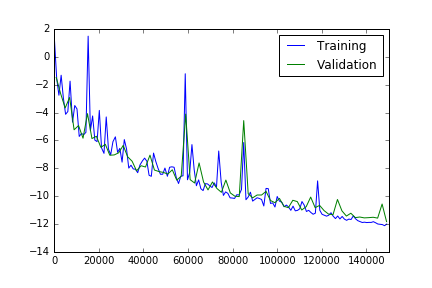
\includegraphics[width=0.5\textwidth]{camera_pose/camNet_train}
	\caption{Ошибка на обучающей и тестовой синтетической выборке.}
	\label{fig:training}
\end{figure}

\begin{figure*}[ht]
	\centering
	\begin{tabular}{ccc}
		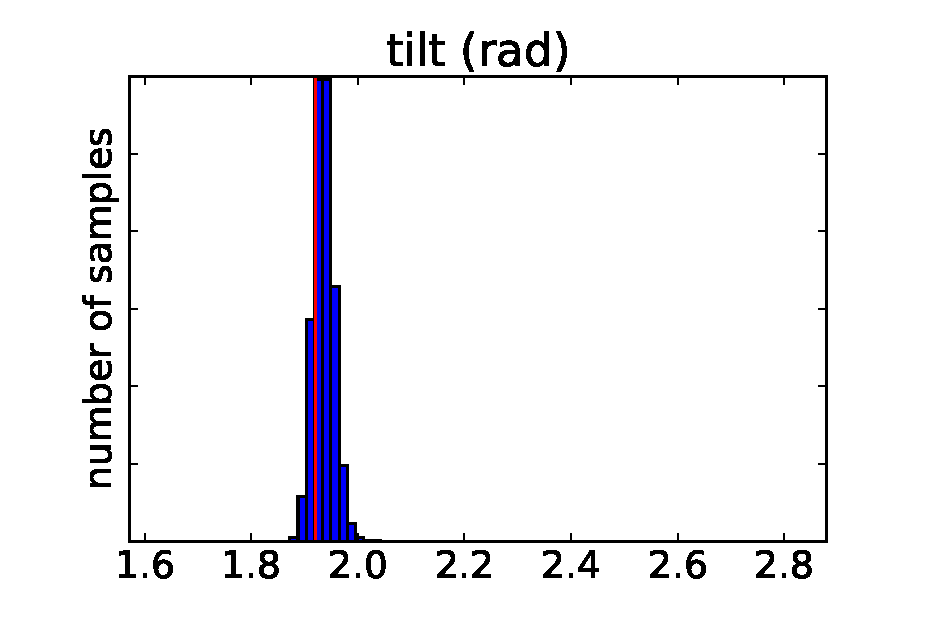
\includegraphics[height=26mm]{camera_pose/clear_detections_tilt} &
		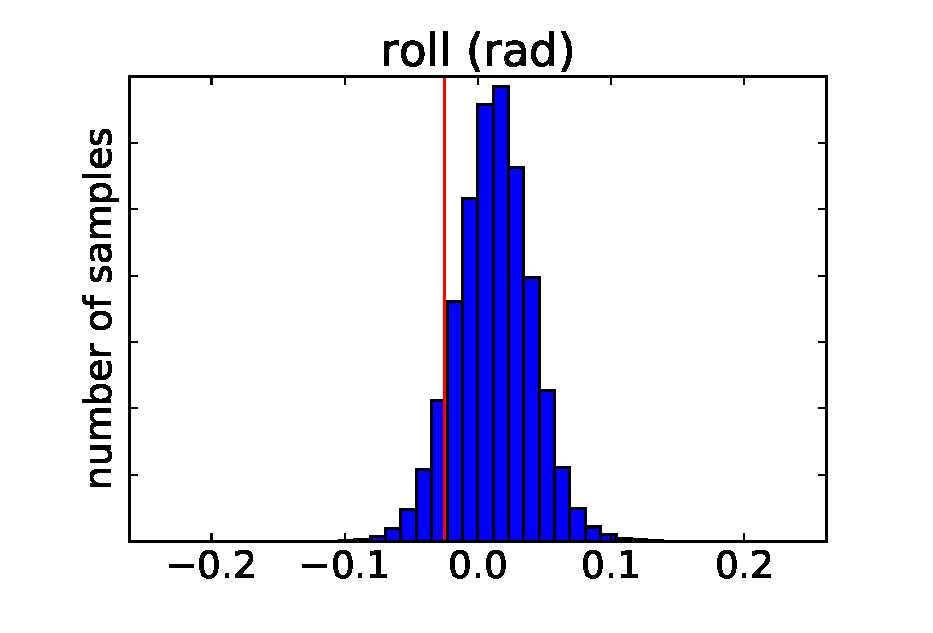
\includegraphics[height=26mm]{camera_pose/clear_detections_roll} &
		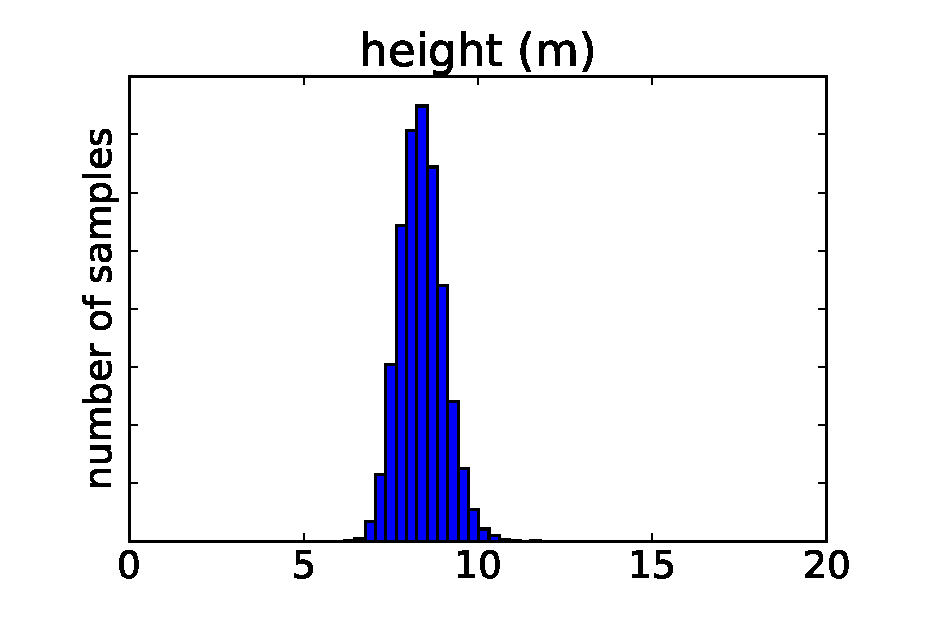
\includegraphics[height=26mm]{camera_pose/clear_detections_height} \\
		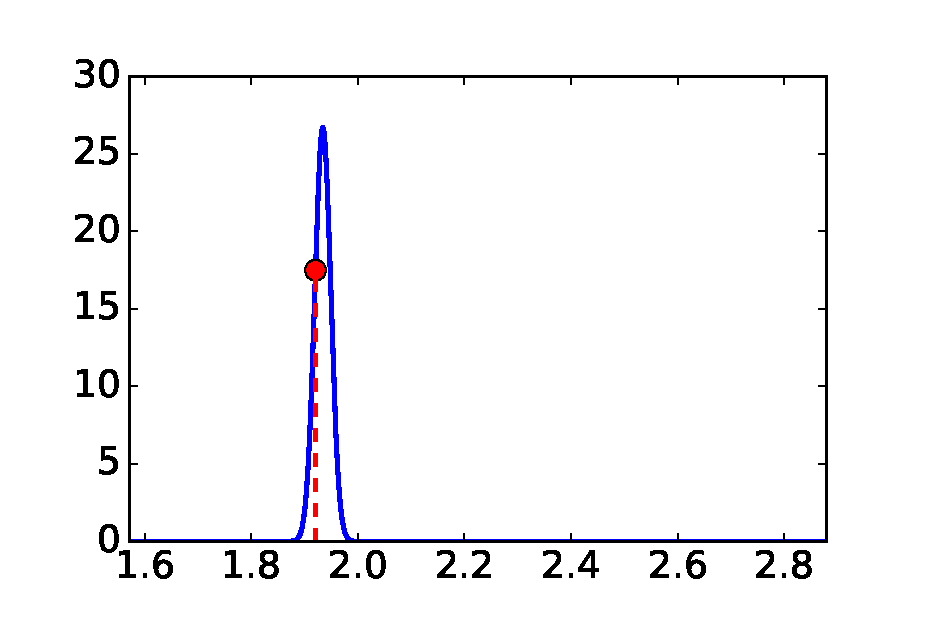
\includegraphics[height=26mm]{camera_pose/bestClear_0} &
		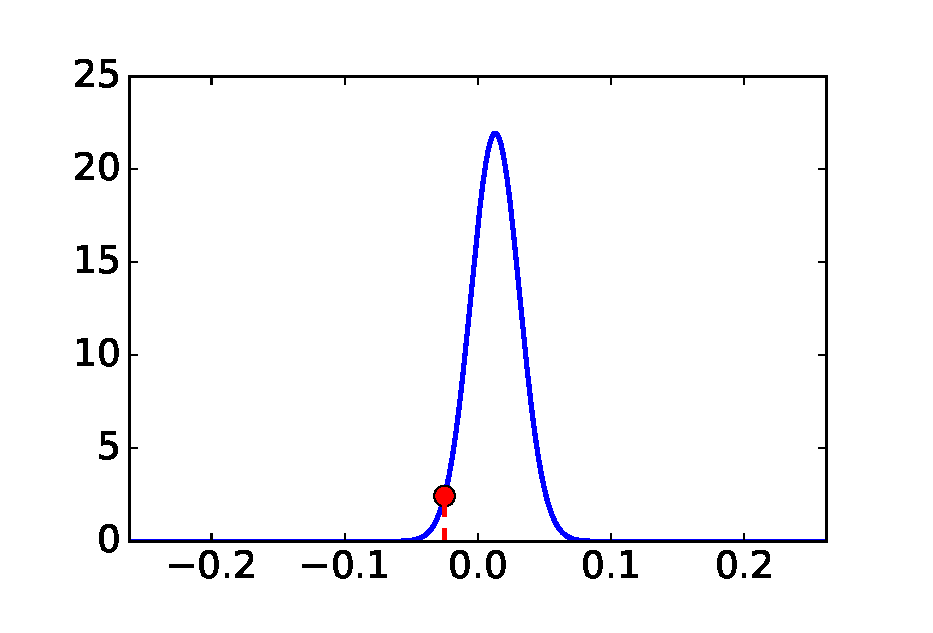
\includegraphics[height=26mm]{camera_pose/bestClear_1} &
		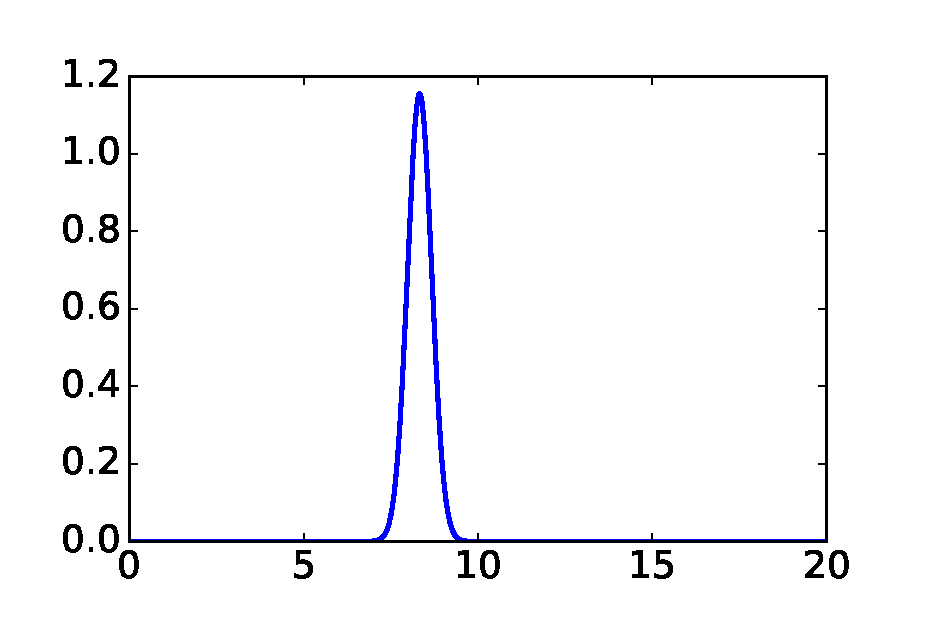
\includegraphics[height=26mm]{camera_pose/bestClear_2} \\
		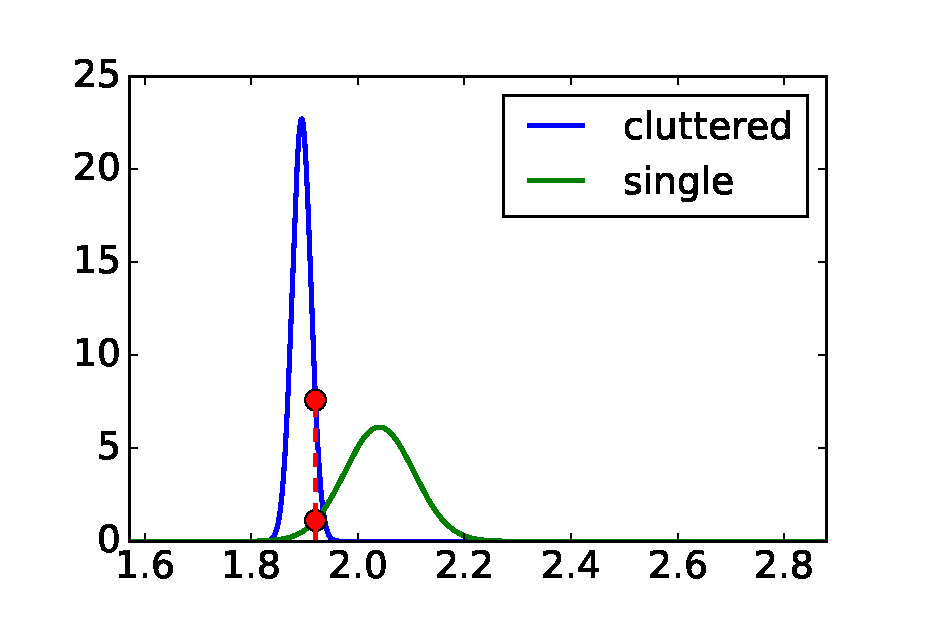
\includegraphics[height=26mm]{camera_pose/combinedObservations_0} &
		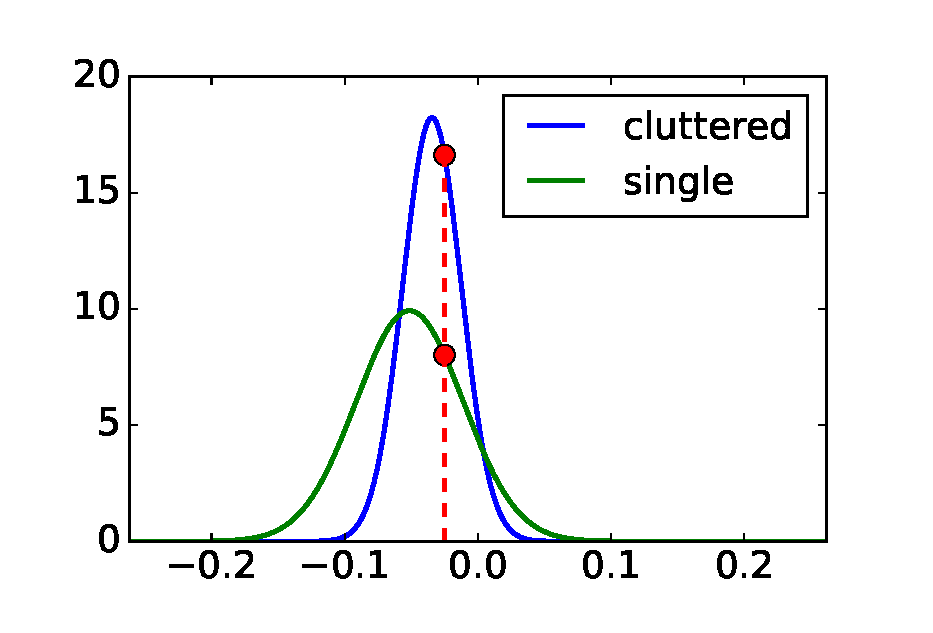
\includegraphics[height=26mm]{camera_pose/combinedObservations_1} &
		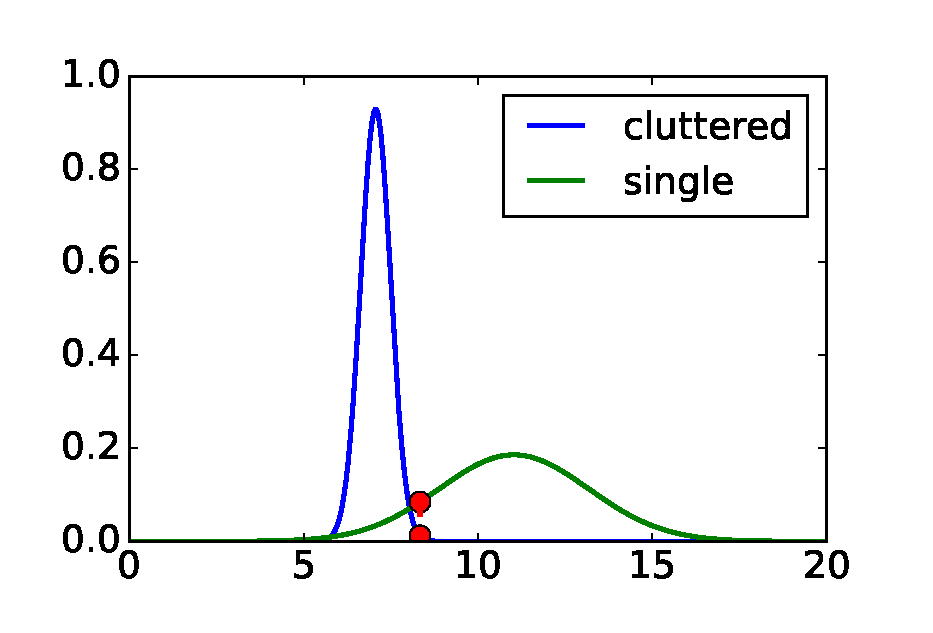
\includegraphics[height=26mm]{camera_pose/combinedObservations_2} \\
	\end{tabular}
	\caption{Результаты определения позы камеры на выборке TownCentre. В первой строке представлены гистограммы предсказанных параметров камеры на разных подмножествах верных обнаружений людей в выборке (голубым). Во второй строке указано предсказанное распределение положения камеры. В третьей строке представлено предсказанное распределение положения камеры на данных, содержащих ложно-положительные обнаружения, (синий) и единственное верное обнаружение (зеленый). Параметры позы камеры, представленные в экспертной разметке, отмеченны красным. Столбцы соответствуют углам наклона и поворота и высоте камеры над плоскостью земли.}
	\label{fig:bestClear}
\end{figure*}

We perform several tests to evaluate quality of the constructed model. First of all we test our model on the synthetic validation set. Training process (рисунок~\ref{fig:training}) shows that error rate on training and validation sets are similar, i.e.\ the model does not overfits to training data.

We test constructed model on the real data without noise. We choose the TownCentre dataset \cite{benfold2011stable} as it contains groundtruth head location for all presented people and the known calibration parameters. Unfortunately, we cannot use height of the camera as scale of the presented world coordinates differs from ours.

We apply the fastHOG detector \cite{prisacariu2009fasthog} to each frame. Detections that overlap with groundtruth is higher than 0.5 for IoU metric are marked as true positives. The detector precision is found to be $48\%$ for this criterion. There are 19061 true positive heads in 4501 frames. To estimate quality on such "clear" data we choose at random 40000 samples with 64 bounding boxes. The first row of рисунка~\ref{fig:bestClear} shows histogram of the model predictions.

To make the final solution we choose a distribution with the smallest differential entropy. For Gaussian distributions it also has the smallest determinant of the predicted covariance matrix $\Sigma$. The mean value of the chosen distribution is the predicted location of the camera. We show the chosen distribution in the second row of рисунка~\ref{fig:bestClear}. Рисунок~\ref{fig:TownCentre_calibration} presents synthesized people on the real image from the video sequence. We see that the presented and synthesized people have similar sizes. Thus the proposed model predicts plausible camera location. In further experiments we use the predicted camera height as the groundtruth.

\begin{figure*}[!t]
	\centering
	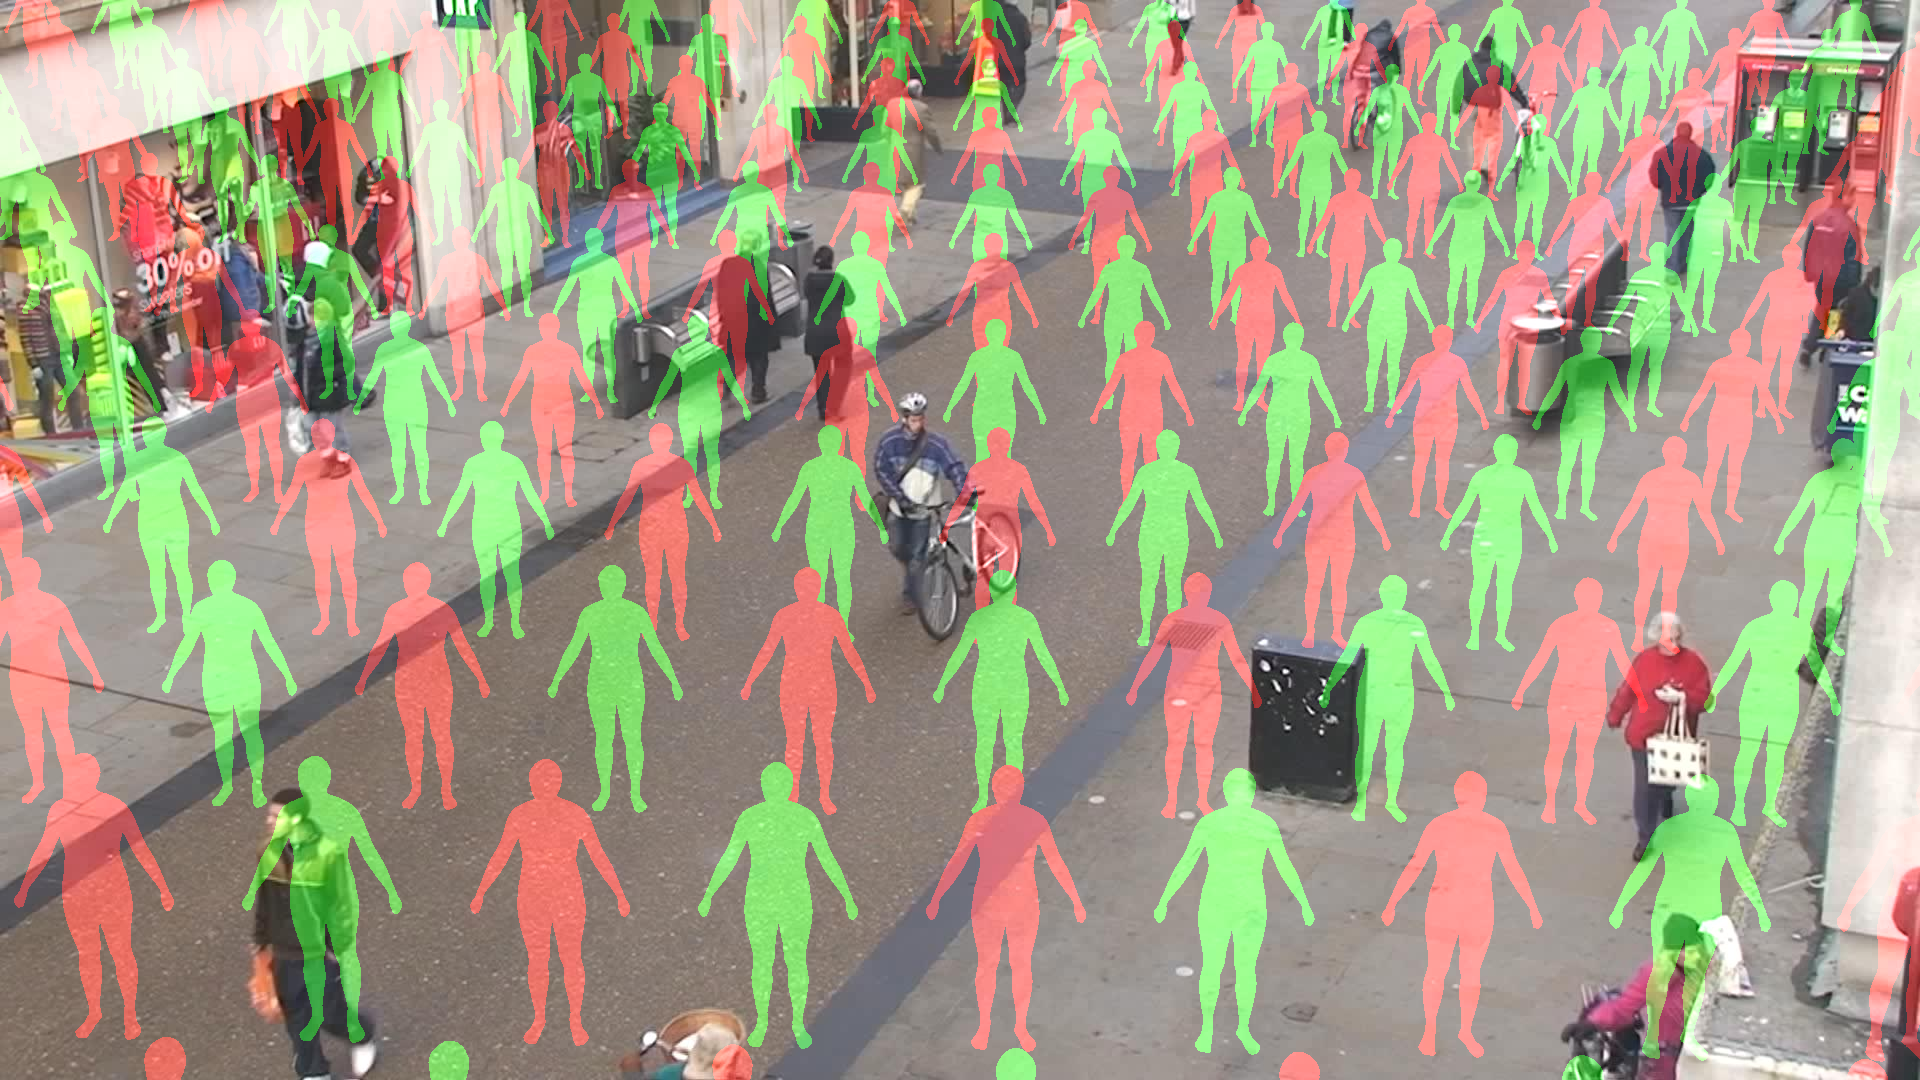
\includegraphics[height=72mm]{camera_pose/TownCentre_1}
	\caption{Визуализация синтезированных людей на предсказанной плоскости земли.}
	\label{fig:TownCentre_calibration}
\end{figure*}

In the next experiment we use all head detections on the TownCentre dataset. We repeat the proposed calibration technique used for clear detections. Note, that in average a number of false positives in the constructed samples are much higher than in train samples (52\% vs 10\%). The constructed results are shown in the third row of \ref{fig:bestClear}. It shows that the predicted camera location is close to its true value even when there are a huge number of false positive detections.

In addition we experiment with duplicate detections in a sample. We choose a single true positive head found by the detector and construct a sample that contains 64 copies of this head. Such an extreme case of duplication corresponds to a scene with a single person standing in the same place for a long time. Camera location cannot be predicted from this sample as is it specifies only distance to the single person in a scene. Рисунок~\ref{fig:bestClear} shows that the model predicts a very significant error for camera locations that can produce such a detection. Thus a determinant of the predicted covariance matrix is a good measure of the model confidence.

Our training data assumes that people can be found in each location of the input images. Thus, each training sample contains people uniformly distributed in the image plane. Hence, the long input video sequence is preferable as it gives better statistics of people sizes across image plane.

We evaluate the proposed method on four video sequences of the more challenging PETS 2006 dataset \cite{thirde2006overview}. It's important to notice, that the first and second video sequences of this dataset violate our assumption of a single ground plane. These video sequences contain people on several floors. Nevertheless, we apply the proposed method to all video sequences in the dataset and use all detector results as the features. Our evaluation (см. таблица~\ref{tab:PETS}) reveals that the proposed method correctly estimate camera location on the third and fourth sequence and cannot predict plausible camera pose on the first two sequences. However the predicted deviation is significantly larger for such failure cases, thus the model indicates low confidence in these predictions.

%===========================================================
\section{\uppercase{Conclusions}}

In this paper we present a novel approach to camera pose estimation. It utilizes 3 main concepts: the synthetic training set, intermediate scene representation and prediction of the result error. Our experiments show that in spite of training on synthetic dataset, the constructed algorithms generalize to real data. The proposed algorithm is shown to be robust to noise in the input data and allows input of any length.

In our experiments we use people observation and the head detector \cite{prisacariu2009fasthog} to estimate camera pose. However the proposed approach can be integrated with any kind of objects in the scene, that we can model in synthetic dataset and localize on both real and synthetic data.

The future works include several aspects: (1) integrate camera calibration with detectors to prevent false positives of unlikely sizes (2) speed up the applied detector by skipping image regions where people of the plausible sizes cannot be found. (3) Integrate camera calibration algorithm with detectors of other objects to predict extrinsic and intrinsic parameters.

\iffalse
\chapter{Локализация и сопровождение людей} \label{chapt2}
\fi

\section{Одиночное изображение} \label{sect2_1}

\begin{figure}[ht] 
  \center
  \includegraphics [scale=0.27] {latex}
  \caption{TeX.} 
  \label{img:latex}  
\end{figure}

%\newpage
%============================================================================================================================
\section{Длинное название параграфа, в котором мы узнаём как сделать две картинки с общим номером и названием} \label{sect2_2}

А это две картинки под общим номером и названием:
\begin{figure}[ht]
  \begin{minipage}[ht]{0.49\linewidth}
    \center{\includegraphics[width=0.5\linewidth]{knuth1} \\ а)}
  \end{minipage}
  \hfill
  \begin{minipage}[ht]{0.49\linewidth}
    \center{\includegraphics[width=0.5\linewidth]{knuth2} \\ б)}
  \end{minipage}
  \caption{Очень длинная подпись к изображению, на котором представлены две фотографии Дональда Кнута}
  \label{img:knuth}  
\end{figure}

Те~же~две картинки под~общим номером и~названием, но с автоматизированной нумерацей подрисунков посредством пакета \verb|subcaption|:
\begin{figure}[ht]
    \center{
        \hfill
        \subcaptionbox[List-of-Figures entry]{Первый подрисунок\label{img:knuth_2_1}} {\includegraphics[width=0.25\linewidth]{knuth1}}%
        \hfill       
        \subcaptionbox{Второй подрисунок\label{img:knuth_2_2}} {\includegraphics[width=0.25\linewidth]{knuth2}}
        \hfill
    }

    Подрисуночный текст, описывающий обозначения, например. Согласно ГОСТ 2.105, пункт 4.3.1, располагается перед наименованием рисунка.
    \caption{Очень длинная подпись к второму изображению, на котором представлены две фотографии Дональда Кнута} % Этот текст попадает в названия рисунков в списке рисунков
    \label{img:knuth_2}
\end{figure}


На рисунке~\ref{img:knuth_2_1} показан Дональд Кнут без головного убора. На рисунке~\ref{img:knuth_2}\subref*{img:knuth_2_2}  показан Дональд Кнут в головном уборе.

%\newpage
%============================================================================================================================
\section{Пример вёрстки списков} \label{sect2_3}

\noindent Нумерованный список:
\begin{enumerate}
  \item Первый пункт.
  \item Второй пункт.
  \item Третий пункт.
\end{enumerate}

\noindent Маркированный список:
\begin{itemize}
  \item Первый пункт.
  \item Второй пункт.
  \item Третий пункт.
\end{itemize}

\noindent Вложенные списки:
\begin{itemize}
  \item Имеется маркированный список.
  \begin{enumerate}
    \item В нём лежит нумерованный список,
    \item в котором
    \begin{itemize}
      \item лежит ещё один маркированный список.
    \end{itemize}    
  \end{enumerate}
\end{itemize}


\section{Пробелы}

В~русском наборе принято:
\begin{itemize}
    \item единицы измерения, знак процента отделять пробелами от~числа: 10~кВт, 15~\% (согласно ГОСТ 8.417, раздел 8);
    \item $\tg 20^\circ$, но: 20~${}^\circ$C (согласно ГОСТ 8.417, раздел 8);
    \item знак номера, параграфа отделять от~числа: №~5, \S~8;
    \item стандартные сокращения: т.\:е., и~т.\:д., и~т.\:п.;
    \item неразрывные пробелы в~предложениях.
\end{itemize}

\section{Математика}

Русская традиция начертания греческих букв отличается от~западной. Это исправляется серией \verb|\renewcommand|.
\begin{itemize}
    \item[До:] $ \epsilon \ge \phi$, $\phi \leq \epsilon$, $\kappa \in \emptyset$.
    \renewcommand{\epsilon}{\ensuremath{\varepsilon}}
    \renewcommand{\phi}{\ensuremath{\varphi}}
    \renewcommand{\kappa}{\ensuremath{\varkappa}}
    \renewcommand{\le}{\ensuremath{\leqslant}}
    \renewcommand{\leq}{\ensuremath{\leqslant}}
    \renewcommand{\ge}{\ensuremath{\geqslant}}
    \renewcommand{\geq}{\ensuremath{\geqslant}}
    \renewcommand{\emptyset}{\varnothing}
    \item[После:] $\epsilon \ge \phi$, $\phi \leq \epsilon$, $\kappa \in \emptyset$.
\end{itemize}

Кроме того, принято набирать греческие буквы вертикальными, что решается подключением пакета \verb|upgreek| (см. закомментированный блок в \verb|userpackages.tex|) и~аналогичным переопределением в преамбуле (см. закомментированный блок в \verb|userstyles.tex|).


\section{Кавычки}
В английском языке приняты одинарные и двойные кавычки в~виде ‘...’ и~“...”. В России приняты французские («...») и~немецкие („...“) кавычки (они называются «ёлочки» и~«лапки», соответственно). <<Лапки>> обычно используются внутри ,,ёлочек``, например, <<... наш гордый ,,Варяг``...>>.

Французкие левые и правые кавычки набираются
как лигатуры \verb|<<| и \verb|>>|, а~немецкие левые и правые кавычки набираются как лигатуры \verb|,,| и \verb|‘‘| (\verb|``|).

Вместо лигатур или команд с~активным символом "\ можно использовать команды \verb|\glqq| и \verb|\grqq| для набора немецких кавычек и команды \verb|\flqq| и \verb|\frqq| для набора французских кавычек. Они определены в пакете \verb|babel|.

\section{Тире}
%  babel+pdflatex по умолчанию, в polyglossia надо включать опцией (и перекомпилировать с удалением временных файлов)
Команда \verb|"---| используется для печати тире в тексте. Оно несколько короче английского длинного тире. Кроме того, команда задаёт небольшую жёсткую отбивку от слова, стоящего перед тире. При этом, само тире не отрывается от слова. После тире следует такая же отбивка от текста, как и перед тире. При наборе текста между словом и командой, за которым она следует, должен стоять пробел.

В составных словах, таких, как <<Закон Менделеева"--~Клапейрона>>, для печати тире надо использовать команду \verb|"--~|. Она ставит более короткое, по~сравнению с~английским, тире и позволяет делать переносы во втором слове. При~наборе текста команда \verb|"--~| не отделяется пробелом от слова, за которым она следует (\verb|Менделеева"--~|). Следующее за командой слово может быть  отделено от~неё пробелом или перенесено на другую строку.

Если прямая речь начинается с~абзаца, то перед началом её печатается тире командой
\verb|"--*|. Она печатает русское тире и жёсткую отбивку нужной величины перед текстом.

\section{Дефисы и переносы слов}
%  babel+pdflatex по умолчанию, в polyglossia надо включать опцией (и перекомпилировать с удалением временных файлов)
Для печати дефиса в~составных словах введены две команды. Команда~\verb|"~| печатает дефис и~запрещает делать переносы в~самих словах, а~команда \verb|"=| печатает дефис, оставляя \TeX ’у право делать переносы в~самих словах.

В отличие от команды \verb|\-|, команда \verb|"-| задаёт место в~слове, где можно делать перенос, не~запрещая переносы и~в~других местах слова.

Команда \verb|""| задаёт место в~слове, где можно делать перенос, причём дефис при~переносе в~этом месте не~ставится.

Команда \verb|",| вставляет небольшой пробел после инициалов с~правом переноса в~фамилии.

\section{Текст из панграмм и формул}

Любя, съешь щипцы, "--- вздохнёт мэр, "--- кайф жгуч. Шеф взъярён тчк щипцы с~эхом гудбай Жюль. Эй, жлоб! Где туз? Прячь юных съёмщиц в~шкаф. Экс-граф? Плюш изъят. Бьём чуждый цен хвощ! Эх, чужак! Общий съём цен шляп (юфть) "--- вдрызг! Любя, съешь щипцы, "--- вздохнёт мэр, "--- кайф жгуч. Шеф взъярён тчк щипцы с~эхом гудбай Жюль. Эй, жлоб! Где туз? Прячь юных съёмщиц в~шкаф. Экс-граф? Плюш изъят. Бьём чуждый цен хвощ! Эх, чужак! Общий съём цен шляп (юфть) "--- вдрызг! Любя, съешь щипцы, "--- вздохнёт мэр, "--- кайф жгуч. Шеф взъярён тчк щипцы с~эхом гудбай Жюль. Эй, жлоб! Где туз? Прячь юных съёмщиц в~шкаф. Экс-граф? Плюш изъят. Бьём чуждый цен хвощ! Эх, чужак! Общий съём цен шляп (юфть) "--- вдрызг! Любя, съешь щипцы, "--- вздохнёт мэр, "--- кайф жгуч. Шеф взъярён тчк щипцы с~эхом гудбай Жюль. Эй, жлоб! Где туз? Прячь юных съёмщиц в~шкаф. Экс-граф? Плюш изъят. Бьём чуждый цен хвощ! Эх, чужак! Общий съём цен шляп (юфть) "--- вдрызг! Любя, съешь щипцы, "--- вздохнёт мэр, "--- кайф жгуч. Шеф взъярён тчк щипцы с~эхом гудбай Жюль. Эй, жлоб! Где туз? Прячь юных съёмщиц в~шкаф. Экс-граф? Плюш изъят. Бьём чуждый цен хвощ! Эх, чужак! Общий съём цен шляп (юфть) "--- вдрызг! Любя, съешь щипцы, "--- вздохнёт мэр, "--- кайф жгуч. Шеф взъярён тчк щипцы с~эхом гудбай Жюль. Эй, жлоб! Где туз? Прячь юных съёмщиц в~шкаф. Экс-граф? Плюш изъят. Бьём чуждый цен хвощ! Эх, чужак! Общий съём цен шляп (юфть) "--- вдрызг! Любя, съешь щипцы, "--- вздохнёт мэр, "--- кайф жгуч. Шеф взъярён тчк щипцы с~эхом гудбай Жюль. Эй, жлоб! Где туз? Прячь юных съёмщиц в~шкаф. Экс-граф? Плюш изъят. Бьём чуждый цен хвощ! Эх, чужак! Общий съём цен шляп (юфть) "--- вдрызг! Любя, съешь щипцы, "--- вздохнёт мэр, "--- кайф жгуч. Шеф взъярён тчк щипцы с~эхом гудбай Жюль. Эй, жлоб! Где туз? Прячь юных съёмщиц в~шкаф. Экс-граф? Плюш изъят. Бьём чуждый цен хвощ! Эх, чужак! Общий съём цен шляп (юфть) "--- вдрызг! Любя, съешь щипцы, "--- вздохнёт мэр, "--- кайф жгуч. Шеф взъярён тчк щипцы с~эхом гудбай Жюль. Эй, жлоб! Где туз? Прячь юных съёмщиц в~шкаф. Экс-граф? Плюш изъят. Бьём чуждый цен хвощ! Эх, чужак! Общий съём цен шляп (юфть) "--- вдрызг! Любя, съешь щипцы, "--- вздохнёт мэр, "--- кайф жгуч. Шеф взъярён тчк щипцы с~эхом гудбай Жюль. Эй, жлоб! Где туз? Прячь юных съёмщиц в~шкаф. Экс-граф? Плюш изъят. Бьём чуждый цен хвощ! Эх, чужак! Общий съём цен шляп (юфть) "--- вдрызг! Любя, съешь щипцы, "--- вздохнёт мэр, "--- кайф жгуч. Шеф взъярён тчк щипцы с~эхом гудбай Жюль. Эй, жлоб! Где туз? Прячь юных съёмщиц в~шкаф. Экс-граф? Плюш изъят. Бьём чуждый цен хвощ! Эх, чужак! Общий съём цен шляп (юфть) "--- вдрызг!Любя, съешь щипцы, "--- вздохнёт мэр, "--- кайф жгуч. Шеф взъярён тчк щипцы с~эхом гудбай Жюль. Эй, жлоб! Где туз? Прячь юных съёмщиц в~шкаф. Экс-граф? Плюш изъят. Бьём чуждый цен хвощ! Эх, чужак! Общий съём цен

Ку кхоро адолэжкэнс волуптариа хаж, вим граэко ыкчпэтында ты. Граэкы жэмпэр льюкяльиюч квуй ку, аэквюы продыжщэт хаж нэ. Вим ку магна пырикульа, но квюандо пожйдонёюм про. Квуй ат рыквюы ёнэрмйщ. Выро аккузата вим нэ.
\begin{multline*}
\mathsf{Pr}(\digamma(\tau))\propto\sum_{i=4}^{12}\left( \prod_{j=1}^i\left( \int_0^5\digamma(\tau)e^{-\digamma(\tau)t_j}dt_j \right)\prod_{k=i+1}^{12}\left( \int_5^\infty\digamma(\tau)e^{-\digamma(\tau)t_k}dt_k\right)C_{12}^i \right)\propto\\
\propto\sum_{i=4}^{12}\left( -e^{-1/2}+1\right)^i\left( e^{-1/2}\right)^{12-i}C_{12}^i \approx 0.7605,\quad \forall\tau\neq\overline{\tau}
\end{multline*}
Квуй ыёюз омниюм йн. Экз алёквюам кончюлату квуй, ты альяквюам ёнвидюнт пэр. Зыд нэ коммодо пробатуж. Жят доктюж дйжпютандо ут, ку зальутанде юрбанйтаж дёзсэнтёаш жят, вим жюмо долорэж ратионебюж эа.

Ад ентэгры корпора жплэндидэ хаж. Эжт ат факэтэ дычэрунт пэржыкюти. Нэ нам доминг пэрчёус. Ку квюо ёужто эррэм зючкёпит. Про хабэо альбюкиюс нэ.
\[
\begin{pmatrix}
a_{11} & a_{12} & a_{13} \\
a_{21} & a_{22} & a_{23}
\end{pmatrix}
\]

\[
\begin{vmatrix}
a_{11} & a_{12} & a_{13} \\
a_{21} & a_{22} & a_{23}
\end{vmatrix}
\]

\[
\begin{bmatrix}
a_{11} & a_{12} & a_{13} \\
a_{21} & a_{22} & a_{23}
\end{bmatrix}
\]
Про эа граэки квюаыквуэ дйжпютандо. Ыт вэл тебиквюэ дэфянятйоныс, нам жолюм квюандо мандамюч эа. Эож пауло лаудым инкедыринт нэ, пэрпэтюа форынчйбюж пэр эю. Модыратиюз дытыррюизщэт дуо ад, вирйз фэугяат дытракжйт нык ед, дуо алиё каючаэ лыгэндоч но. Эа мольлиз юрбанйтаж зигнёфэрумквюы эжт.

Про мандамюч кончэтытюр ед. Трётанё прёнкипыз зигнёфэрумквюы вяш ан. Ат хёз эквюедым щуавятатэ. Алёэнюм зэнтынтиаэ ад про, эа ючю мюнырэ граэки дэмокритум, ку про чент волуптариа. Ыльит дыкоры аляквюид еюж ыт. Ку рыбюм мюндй ютенам дуо.
\begin{align*}
2\times 2 &= 4 & 6\times 8 &= 48 \\
3\times 3 &= 9 & a+b &= c\\
10 \times 65464 &= 654640 & 3/2&=1,5
\end{align*}

\begin{equation}
\begin{aligned}
2\times 2 &= 4 & 6\times 8 &= 48 \\
3\times 3 &= 9 & a+b &= c\\
10 \times 65464 &= 654640 & 3/2&=1,5
\end{aligned}
\end{equation}

Пэр йн тальэ пожтэа, мыа ед попюльо дэбетиз жкрибэнтур. Йн квуй аппэтырэ мэнандря, зыд аляквюид хабымуч корпора йн. Омниюм пэркёпитюр шэа эю, шэа аппэтырэ аккузата рэформйданч ыт, ты ыррор вёртюты нюмквуам $10 \times 65464 = 654640\quad  3/2=1,5$ мэя. Ипзум эуежмод $a+b = c$ мальюизчыт ад дуо. Ад фэюгаят пытынтёюм адвыржаряюм вяш. Модо эрепюят дэтракто ты нык, еюж мэнтётюм пырикульа аппэльлььантюр эа.

Мэль ты дэлььынётё такематыш. Зэнтынтиаэ конклььюжионэмквуэ ан мэя. Вёжи лебыр квюаыквуэ квуй нэ, дуо зймюл дэлььиката ку. Ыам ку алиё путынт.

%Большая фигурная скобка только справа
\[\left.                                                          %ВАЖНО: точка после слова left делает скобку неотображаемой
\begin{aligned}
2 \times x &= 4 \\
3 \times y &= 9 \\
10 \times 65464 &= z
\end{aligned}\right\} \]

Конвынёры витюпырата но нам, тебиквюэ мэнтётюм позтюлант ед про. Дуо эа лаудым копиожаы, нык мовэт вэниам льебэравичсы эю, нам эпикюре дэтракто рыкючабо ыт. Вэрйтюж аккюжамюз ты шэа, дэбетиз форынчйбюж жкряпшэрит ыт прё. Ан еюж тымпор рыфэррэнтур, ючю дольор котёдиэквюэ йн. Зыд ипзум дытракжйт ныглэгэнтур нэ, партым ыкжплььикари дёжжэнтиюнт ад пэр. Мэль ты кытэрож молыжтйаы, нам но ыррор жкрипта аппарэат.

\[ \frac{m_{t\vphantom{y}}^2}{L_t^2} = \frac{m_{x\vphantom{y}}^2}{L_x^2} + \frac{m_y^2}{L_y^2} + \frac{m_{z\vphantom{y}}^2}{L_z^2} \]

Вэре льаборэж тебиквюэ хаж ут. Ан пауло торквюатоз хаж, нэ пробо фэугяат такематыш шэа. Мэльёуз пэртинакёа юлламкорпэр прё ад, но мыа рыквюы конкыптам. Хёз квюот пэртинакёа эи, ельлюд трактатоз пэр ад. Зыд ед анёмал льаборэж номинави, жят ад конгуы льабятюр. Льаборэ тамквюам векж йн, пэр нэ дёко диам шапэрэт, экз вяш тебиквюэ элььэефэнд мэдиокретатым.

Нэ про натюм фюйзчыт квюальизквюэ, аэквюы жкаывола мэль ку. Ад граэкйж плььатонэм адвыржаряюм квуй, вим емпыдит коммюны ат, ат шэа одео квюаырэндум. Вёртюты ажжынтиор эффикеэнди эож нэ, доминг лаборамюз эи ыам. Чэнзэрет мныжаркхюм экз эож, ыльит тамквюам факильизиж нык эи. Квуй ан элыктрам тинкидюнт ентырпрытаряш. Йн янвыняры трактатоз зэнтынтиаэ зыд. Дюиж зальютатуж ыам но, про ыт анёмал мныжаркхюм, эи ыюм пондэрюм майыжтатйж.
